% Canonical Companion Part IV source figure
% Companion problem: CP-IV-0066
% Source problem: IMP-DL-D4351A3BBD-P021
% Source: 1681-L1733
% This file preserves the source TikZ/figure block verbatim except for this provenance header.
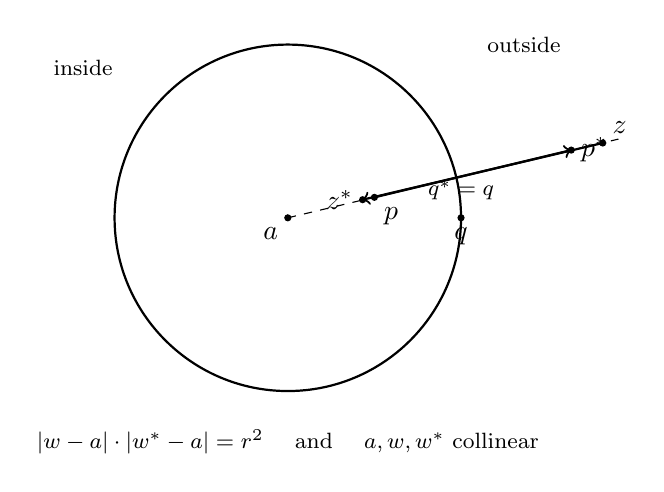
\begin{tikzpicture}[scale=1.0]
		\coordinate (A) at (0,0);
		\def\r{2.2}
		
		% circle
		\draw[thick] (A) circle (\r);
		\fill (A) circle (1.3pt) node[below left] {$a$};
		
		% point on circle (fixed)
		\coordinate (Q) at (\r,0);
		\fill (Q) circle (1.3pt) node[below] {$q$};
		\node at (\r,0.35) {\footnotesize $q^{*}=q$};
		
		% choose a ray direction
		\coordinate (Dir) at (4.2,1.0);
		\draw[dashed] (A) -- (Dir);
		
		% inside point p and its image p*
		\coordinate (P)  at (1.1,0.26);   % inside
		\coordinate (Ps) at (3.6,0.86);   % outside (schematic position)
		\fill (P)  circle (1.3pt) node[below right] {$p$};
		\fill (Ps) circle (1.3pt) node[right] {$p^{*}$};
		\draw[->,thick] (P) -- (Ps);
		
		% outside point z and its image z*
		\coordinate (Z)  at (4.0,0.95);   % outside
		\coordinate (Zs) at (0.95,0.23);  % inside (schematic position)
		\fill (Z)  circle (1.3pt) node[above right] {$z$};
		\fill (Zs) circle (1.3pt) node[left] {$z^{*}$};
		\draw[->,thick] (Z) -- (Zs);
		
		% labels
		\node at (0,-2.85) {\footnotesize $|w-a|\cdot|w^{*}-a|=r^{2}$ \quad and \quad $a,w,w^{*}$ collinear};
		\node at (-2.6,1.9) {\footnotesize inside};
		\node at ( 3.0,2.2) {\footnotesize outside};
	\end{tikzpicture}
